\documentclass[10pt,twocolumn,a4paper]{article}
\usepackage[margin=1.8cm,columnsep=0.6cm]{geometry}
\usepackage{amsmath,amssymb,booktabs,graphicx,xcolor,hyperref,enumitem,caption,float,microtype}
\usepackage{tikz}
\usepackage{verbatim}
\usetikzlibrary{positioning,arrows.meta,fit}
\hypersetup{colorlinks,linkcolor=black,citecolor=black,urlcolor=blue!50!black}
\setlist{itemsep=1pt,topsep=2pt,leftmargin=*}
\captionsetup{font=small,labelfont=bf}
\renewcommand{\arraystretch}{1.12}
\newcommand{\pp}{\,pp}

\title{\textbf{A Fully Integer, Subject-Independent sEMG Gesture Classifier ASIC:\\
Design Decisions, Trade-offs and Verification}}
\author{Vinay Hariharan, Sudhindra, Yash, Digvijay\\
\small Department of Electrical Engineering, IIT Bombay \quad Advisor: Prof.\ Laxmeesha Somappa (BioNICS)\\
\small B.Tech project report, November 2026}
\date{}

\begin{document}
\maketitle

\begin{abstract}
We designed and verified a fixed-function digital core that classifies four hand and wrist gestures
from 8 to 24 surface-EMG electrodes using only integer arithmetic and one $8\times8$ multiplier.
Every design choice was settled by a measured, subject-independent experiment on the public
FORS-EMG dataset (leave-one-subject-out, paired statistics). The choice of gesture set was the
largest single factor (+14.1\pp). Classifier capacity did not matter: an MLP, logistic regression
and LDA are statistically tied, and INT8 quantisation costs 0.18\pp\ on average. Replacing
floating-point features with add, compare and shift operations and a shift normaliser costs no
accuracy (77.79\% vs 77.88\%). The resulting INT8 LDA core is described in synthesisable
Verilog. A bit-exact golden model reproduces the software accuracy (77.61\% vs 77.83\%, no
detectable difference), and the RTL matches that golden model bit for bit at every channel count
from 8 to 24, using at most 850 of the 1015 clock cycles available per sample. We also report the
alternatives we evaluated and rejected (CNNs, trees, hyperdimensional computing, Tsetlin machines,
compute-in-memory), per-user calibration, which recovers the worst users, and a sequential
decision rule derived from correlated best-arm identification, which cuts per-decision errors
from 6.6\% to below 1.1\% on five of six gesture pairs.
\end{abstract}

%=======================================================================
\section{Introduction}
Wearable myoelectric control (prostheses, gesture interfaces) needs a classifier that runs
continuously at microwatt power and works for a person it was never trained on. These two
requirements drive every decision in this report.
\begin{itemize}
\item \textbf{Low power} favours integer arithmetic, few multiplications, small memories and a low
clock rate (here 1\,MHz).
\item \textbf{Generalisation to a new user} is the hard part of sEMG classification: skin, fat,
electrode placement and muscle physiology change the signal between people. We therefore report
only subject-independent accuracy.
\end{itemize}
The project went through four phases: choosing the gesture set and classifier
(Sections~\ref{sec:gestures}--\ref{sec:quant}), making the front end integer-only
(Section~\ref{sec:frontend}), designing and verifying the hardware
(Sections~\ref{sec:hw}--\ref{sec:verif}), and evaluating alternatives
(Section~\ref{sec:explore}). Section~\ref{sec:tradeoffs} collects every decision, the
alternatives and the evidence in one table.

%=======================================================================
\section{Dataset and evaluation protocol}\label{sec:protocol}
\textbf{Data.} FORS-EMG: 19 subjects, 8 forearm electrodes, 985\,Hz, 12 gestures in 3 forearm
orientations, 5 trials each; every recording is 8000 samples ($\approx$8.1\,s).

\textbf{Signal chain.} A 20--450\,Hz Butterworth band-pass and a 50\,Hz notch ($Q=30$). The
filter is causal (forward only), because hardware cannot run the zero-phase filter used in the
first experiments: zero-phase filtering applies $|H|^2$ and uses future samples.

\textbf{Windows.} 200\,ms windows (196--197 samples) with a 100\,ms stride.

\textbf{Split.} Leave-one-subject-out (LOSO): the held-out subject is never seen in training,
normalisation or calibration. Within the training subjects, trial 5 is the validation set and
trials 1--4 train. Windows are cut \emph{after} the split. An early bug cut windows first; because
neighbouring windows share half their samples, this leaked validation data into training and
produced a false 63\% ceiling that did not depend on model capacity.

\textbf{Statistics.} Accuracy is the mean over held-out subjects with a 95\% confidence interval.
Two methods are compared per subject (paired): mean difference, 95\% CI of the difference, and the
Wilcoxon signed-rank test. A difference is called real only if its CI excludes zero.

The repository copy of the dataset is missing Subject~1, so runs made for this report use 18
subjects; runs made on the full dataset use 19. Every table states which.

%=======================================================================
\section{Gesture set}\label{sec:gestures}
The first set, \{Hand Close, Hand Open, Index, Index Little\}, stopped at about 65\% whatever the
model (Table~\ref{tab:gestures}). Its confusion matrix showed that Index $\leftrightarrow$ Index
Little alone caused about 40\% of all errors. These two finger movements recruit overlapping deep
flexor compartments, which 8 surface electrodes cannot separate.

\textbf{Decision.} Use \{Hand Close, Hand Open, Wrist Flexion, Wrist Extension\}: gross hand and
wrist movements driven by distinct, superficial muscles. This gained \textbf{+14.1\pp} (paired
$t$-test $p=3.8\times10^{-9}$), more than any later model or hardware choice. Larger vocabularies
cost accuracy: 69.0\% for the best 6 gestures and 48.8\% for all 12 (Fig.~\ref{fig:gestures}). The
remaining dominant confusion, Hand Open $\leftrightarrow$ Wrist Extension, comes from shared
extensor-digitorum activity.

\begin{table}[t]\centering\small
\caption{INT8 LOSO accuracy by gesture vocabulary (19 subjects; best tied model).}\label{tab:gestures}
\resizebox{\linewidth}{!}{%
\begin{tabular}{lccc}\toprule
Gesture set & Accuracy & Chance & $\times$ chance\\\midrule
A: 4 incl.\ Index, Index Little & 65.3\% & 25\% & 2.6\\
\textbf{B: 4 selected (final)} & \textbf{79.4\%} & 25\% & 3.2\\
D: best 6 of 12 & 69.0\% & 16.7\% & 4.1\\
C: all 12 & 48.8\% & 8.3\% & 5.9\\\bottomrule
\end{tabular}}
\end{table}

\begin{figure}[t]\centering
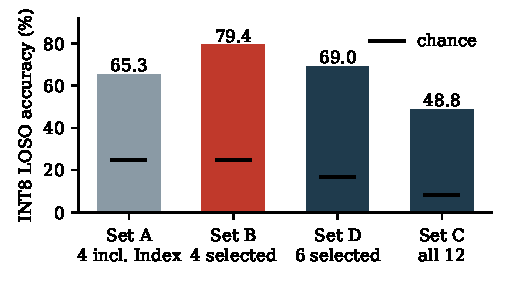
\includegraphics[width=\linewidth]{figures/gesture_sets.pdf}
\caption{Accuracy for each gesture vocabulary; black ticks mark chance level.}\label{fig:gestures}
\end{figure}

The 6-gesture subset was chosen by ranking all $\binom{12}{6}=924$ subsets by their worst pairwise
confusion, using the 12-class confusion matrices. The predicted accuracy (66.4\%, band 65--75\%)
contained the measured 69.0\%, so existing confusion data can rank vocabularies without retraining.

%=======================================================================
\section{Classifier}\label{sec:classifier}
Eight classifiers were trained under one protocol on Gesture Set B, using 64 float features
(8 types $\times$ 8 channels). The memory budget was 10\,KB (Table~\ref{tab:clf}, Fig.~\ref{fig:clf}).

\begin{table}[t]\centering\small
\caption{Classifiers on Gesture Set B (INT8, LOSO, 19 subjects). ``Tied'': paired test against the MLP not significant.}\label{tab:clf}
\resizebox{\linewidth}{!}{%
\begin{tabular}{lrrrl}\toprule
Model & INT8 \% & MACs & Bytes & vs MLP\\\midrule
MLP 64-16-4 & 79.57 & 1088 & 1168 & --\\
Hist.\ grad.\ boosting & 79.26 & 0 & 19\,200 & tied, $>$10\,KB\\
Logistic regression & 79.19 & 256 & 272 & tied\\
Linear SVM & 78.30 & 256 & 272 & tied\\
LDA & 77.87 & 256 & 272 & tied ($p=0.09$)\\
Random forest & 77.43 & 0 & 53\,145 & worse, $>$10\,KB\\
Extra trees & 76.04 & 0 & 38\,015 & worse, $>$10\,KB\\
Decision tree & 73.17 & 0 & 5055 & worse\\\bottomrule
\end{tabular}}
\end{table}

\begin{figure}[t]\centering
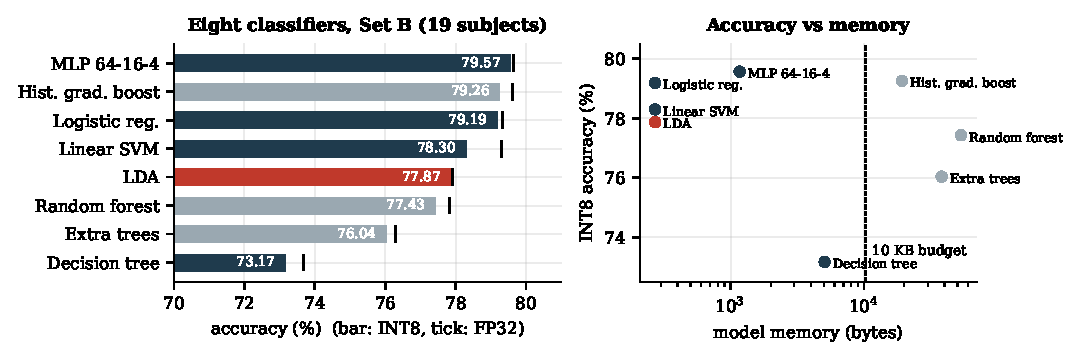
\includegraphics[width=\linewidth]{figures/classifiers.pdf}
\caption{Accuracy against model memory. Grey: over the 10\,KB budget. Red: the chosen LDA.}\label{fig:clf}
\end{figure}

\textbf{Finding: capacity is not the bottleneck.} Five MLP widths (linear up to 64-128-4) were
statistically indistinguishable on Set A. Logistic regression tied the MLP on the 4-, 6- and
12-gesture sets. The limit is the information in surface EMG, not the model.

\textbf{Decision: LDA for the chip.} Logistic regression had the best point estimate among the
cheap models. We still chose LDA, for three reasons that matter in hardware:
\begin{enumerate}
\item its training is closed-form (class means and one shared covariance), with no iterative
optimiser, so it can be retrained or adapted with a few matrix operations;
\item per-user calibration has a closed form too: blend the class means and covariance with the
new user's, then recompute $W$ and $b$ (Section~\ref{sec:calib});
\item its scores have a probabilistic meaning (log-likelihoods up to a shared constant), which the
sequential decision rule of Section~\ref{sec:ctbai} uses.
\end{enumerate}
Its cost is 1.7\pp\ against the MLP, within the tie ($p=0.09$). Trees were excluded: the accurate
ones break the memory budget, and the only one inside it is significantly worse.

%=======================================================================
\section{INT8 quantisation}\label{sec:quant}
Weights and activations are symmetric per-tensor INT8, with biases in INT32 on the same scale.
Across 28 FP32-vs-INT8 comparisons (all models and gesture sets), the mean accuracy loss was
\textbf{0.18\pp} (median 0.11, maximum 1.01 for the linear SVM). Twenty-five of the 28 losses were
under 0.5\pp. A requantisation bug (an undefined shift when the multiplier exceeds 1) would have
cost over 50\pp; a synthetic unit test caught it before any result was reported.

For a classifier that only needs $\arg\max$, requantisation is unnecessary. If every class
score shares one positive scale $s>0$, then
\[
\arg\max_k s\,S_k=\arg\max_k S_k ,
\]
so the chip keeps one INT32 accumulator per class and never rescales. This requires a single
weight scale for all classes.

%=======================================================================
\section{Integer front end}\label{sec:frontend}
The float features (MAV, WL, ZC, SSC, VAR) need division, square roots and floating-point
thresholds. We rebuilt them from operations an ASIC does cheaply: add, subtract, absolute value,
compare, shift, and a leading-one detector.
\begin{itemize}
\item \textbf{SABS} $=\sum|x|$ replaces MAV. The $1/N$ factor is absorbed by normalisation, since
LDA is invariant to rescaling individual features.
\item \textbf{WL} $=\sum|x_n-x_{n-1}|$.
\item \textbf{ZC}: sign-bit XOR of consecutive samples, with no amplitude dead-band (\texttt{ZC\_NODB}).
\item \textbf{SSC}: strict sign change of consecutive differences; only the sign of the previous
difference is stored, so each channel's history needs 10 bits.
\item \textbf{POW}: $\sum x^2$ with Mitchell's one-step approximation of the square,
\[
a^2\approx a\cdot2^{p+1}-2^{2p},\qquad p=\lfloor\log_2 a\rfloor ,
\]
which is one leading-one detector, two shifts and one subtraction, never overestimates, and has
correlation $r=0.9999$ with the exact sum.
\end{itemize}
Log-amplitude features were rejected because a logarithm is expensive in hardware.

\textbf{Normaliser.} Z-scoring and float input quantisation are replaced by
\[
q_f=\operatorname{clip}\!\big(((x_f-\mu_f)+2^{k_f-1})\gg k_f,\;-128,\;127\big),
\]
with integer $\mu_f$ and $k_f$ calibrated on the training subjects.

\textbf{Result.} Six integer variants (H1--H6) were compared against the float reference on the
same folds. Table~\ref{tab:hw} lists the results (18 subjects). With the integer normaliser, every variant
that keeps a power feature is non-inferior to the float reference (margin $-1$\pp). Dropping the
power term (H5) loses about 2\pp, so a power feature is required. Mitchell-1 squares (H3, H6) cost
nothing measurable against exact squares.

\textbf{Decision}: H6, the cheapest variant, with the integer normaliser. On 19 subjects this
fully integer front end gives 77.79$\pm$4.39\% against 77.88\% for the float pipeline.

\begin{table}[t]\centering\small
\caption{Integer feature sets, INT8 LDA, LOSO (18 subjects). $\Delta$: paired difference to R with the shift normaliser, 95\% CI.}\label{tab:hw}
\resizebox{\linewidth}{!}{%
\begin{tabular}{llcc}\toprule
 & Power / ZC variant & Shift norm.\ \% & $\Delta$ vs R (pp)\\\midrule
R & float reference & 77.45 (std) & --\\
H1 & exact $\sum x^2$ & 77.63 & $+0.19$ $[-0.36,+0.73]$\\
H2 & Mitchell-2 & 77.56 & $+0.11$ $[-0.41,+0.63]$\\
H3 & Mitchell-1 & 77.39 & $-0.05$ $[-0.57,+0.47]$\\
H4 & $(\sum|x|)^2$ & 77.14 & $-0.31$ $[-0.88,+0.27]$\\
H5 & no power term & 75.54 & $-1.91$ $[-2.94,-0.87]$\\
\textbf{H6} & \textbf{Mitchell-1, ZC no dead-band} & \textbf{77.39} & $-0.05$ $[-0.59,+0.48]$\\\bottomrule
\end{tabular}}
\end{table}

%=======================================================================
\section{Hardware architecture}\label{sec:hw}
\subsection{System partition}
The question was how to support 8, 12, 16 or 24 electrodes. We considered three options: several
compute boards exchanging partial LDA scores (exact, since the score is a sum over features),
master/slave boards sharing state, or one compute core with pluggable acquisition pods.
A compute-budget analysis settled it. At 1\,MHz, features take about 25 cycles per channel per
sample, so one core handles up to 40 channels within the 1000-cycle sample period, and the LDA
needs $6(D+1)$ cycles per decision. Distributing the computation saves nothing and adds
synchronisation. \textbf{Decision}: one compute core plus 1--3 daisy-chained 8-channel ADC pods,
with the channel count set by one register. Electrodes stay close to the muscle (short leads,
less mains pickup), while all digital work stays on one chip.

\subsection{Datapath}
The datapath has three stages, all on \texttt{clk\_sys} = 1\,MHz (Fig.~\ref{fig:arch}).
\begin{enumerate}
\item \textbf{Stage 1, features} (\texttt{emg\_feat\_accum}). For every frame of $C$ samples, a
two-stage pipeline reads the channel's history and current bank word from RAM, computes the five
features combinationally and writes the updated sums back: $C$ cycles per sample. Two ping-pong
banks of 98 samples give the 196-sample window with a 98-sample stride and a single write
pointer; a window is bank 0 + bank 1.
\item \textbf{Stage 2, normaliser} (\texttt{emg\_shift\_norm}). After every 98th sample, for each
feature it adds the two bank fields, subtracts $\mu_f$, rounds, shifts by $k_f$ and clips:
$D+2$ cycles, with a 24-bit signed datapath derived from the field widths.
\item \textbf{Stage 3, LDA} (\texttt{emg\_lda\_mac}). One signed $8\times8$ multiplier and an
INT32 accumulator. Per class, it loads the bias, then performs $D$ MACs, with one weight-address
counter for all classes (so no $\text{class}\times D$ multiplication). A streaming argmax with
strict $>$ (ties keep the lower class) replaces a comparator tree. Total $6(D+1)+2$ cycles; unused
class slots get bias $-2^{31}$.
\end{enumerate}

\begin{figure}[t]\centering\footnotesize
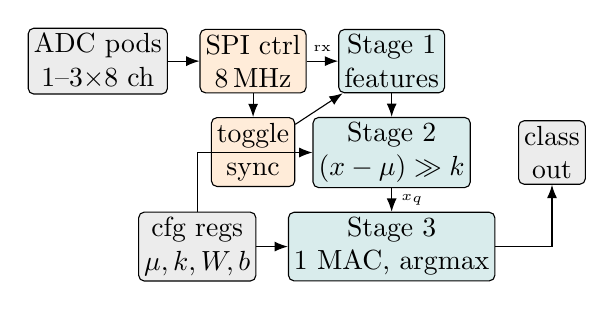
\begin{tikzpicture}[node distance=3mm and 4mm, b/.style={draw,rounded corners=2pt,align=center,minimum height=7mm,inner sep=2pt,fill=#1}, b/.default=white, a/.style={-Latex}]
\node[b=gray!15] (adc) {ADC pods\\1--3$\times$8 ch};
\node[b=orange!15, right=of adc] (spi) {SPI ctrl\\8\,MHz};
\node[b=orange!15, below=of spi] (cdc) {toggle\\sync};
\node[b=teal!15, right=of spi] (s1) {Stage 1\\features};
\node[b=teal!15, below=of s1] (s2) {Stage 2\\$(x-\mu)\gg k$};
\node[b=teal!15, below=of s2] (s3) {Stage 3\\1 MAC, argmax};
\node[b=gray!15, left=of s3] (cfg) {cfg regs\\$\mu,k,W,b$};
\node[b=gray!15, right=6mm of s2] (out) {class\\out};
\draw[a] (adc)--(spi); \draw[a] (spi)--node[above]{\tiny rx} (s1); \draw[a] (spi)--(cdc); \draw[a] (cdc)--(s1);
\draw[a] (s1)--(s2); \draw[a] (s2)--node[right]{\tiny $x_q$} (s3); \draw[a] (cfg)--(s3); \draw[a] (cfg.north)|-(s2.west);
\draw[a] (s3.east)-|(out.south);
\end{tikzpicture}
\caption{Chip partition. Orange: 8\,MHz ADC domain. Teal: the 1\,MHz datapath.}\label{fig:arch}
\end{figure}

\subsection{Clocking, crossing and reset}
The ADC interface runs on an 8\,MHz \texttt{clk\_spi}. It generates CONVST every 8120 cycles
(985\,Hz), detects the fall of DRDY through a 2-flip-flop synchroniser, and reads $8C$ bits at
4\,MHz. Only one event crosses into the core: a frame toggle, through a 2-flip-flop toggle
synchroniser. The data (\texttt{rx\_flat}) crosses unsynchronised, because it is stable for about
1\,ms around the event; in static timing analysis it is declared a multicycle path. Each domain has
its own reset synchroniser (asynchronous assert, synchronous release). Constants and settings are
loaded through one write port into writable memories, not ROM, because every channel count and
electrode layout needs its own trained model.

\subsection{Timing budget}
Stage 1 costs $C$ cycles on every sample. Stages 2 and 3 run once per 98 samples, and their measured
cost grows by 35 cycles per channel, from 290 to 850 (Fig.~\ref{fig:cycles}). Even at 24 channels,
everything finishes within one 1015-cycle sample period. A single multiplier therefore suffices,
and parallel MACs would buy nothing.

\begin{figure}[t]\centering
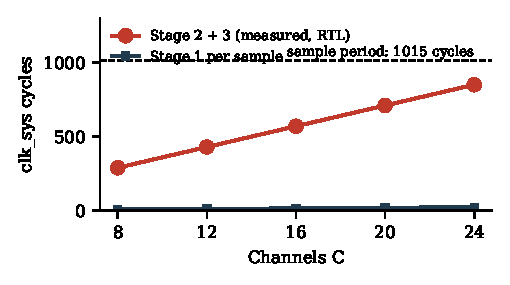
\includegraphics[width=\linewidth]{figures/cycles.pdf}
\caption{Cycle budget against channel count (RTL simulation, $\texttt{clk\_sys}=1$\,MHz).}\label{fig:cycles}
\end{figure}

\subsection{Memory}
\begin{itemize}
\item feature history: $24\times10$ bits;
\item feature banks: $2\times24\times64$ bits;
\item $x_q$: $120\times8$ bits;
\item normaliser constants: $120\times27$ bits;
\item weights: $720\times8$ bits;
\item biases: $6\times32$ bits.
\end{itemize}
The total is about 13.3\,kbit, sized for the worst case of 24 channels and 6 classes. Every
memory has a 1-cycle synchronous read, so the RTL maps to SRAM macros or to flip-flops unchanged.

%=======================================================================
\section{Verification}\label{sec:verif}
\textbf{Golden model.} \texttt{lda\_golden\_model.py} reproduces every integer of Stages 1--3 in
two forms: a sample-by-sample model that mirrors the RTL's counters, and a vectorised model used
for training. The two are cross-checked on every run. Training uses the model's own bit-exact
features, so training and hardware see identical numbers.

\textbf{Does the chip arithmetic cost accuracy?} The golden model (8-bit ADC, streamed
196-sample windows, shift normaliser, single weight scale) was compared with the software INT8 LDA
on the same folds. Result: 77.61$\pm$4.34\% against 77.83$\pm$4.11\%, a difference of
$-0.21$\pp\ with 95\% CI $[-0.72,+0.30]$ and $p=0.49$, so \textbf{no detectable difference}
(18 subjects). The ranges actually used on real data leave wide margins:
\begin{itemize}
\item $\mu_f$: at most 13 of its 22 bits;
\item $|S|$: at most 4047, against the INT32 limit.
\end{itemize}

\textbf{Unit tests.} The feature ALU was tested exhaustively on all 196\,608 input combinations
(every pair of INT8 values, each with the three signs of the previous difference). Each stage
also had its own testbench. We checked that the testbenches catch real bugs by inserting
deliberate ones: a logical instead of arithmetic shift, a missing rounding term, a wrong field, an
unsigned multiply, $\geq$ instead of $>$, a dropped bias and a too-narrow accumulator. All were
caught.

\textbf{Chip-level test.} A cocotb testbench (\texttt{RTL/tb/test\_emg\_top.py}) runs these steps:
\begin{enumerate}
\item it trains a model with the golden model and loads it through the configuration port;
\item it drives an ADC daisy-chain model with a gesture stream at the real clock rates;
\item at every stride it compares the $D$ values of $x_q$, the six class scores and the decided
class against the golden model;
\item it checks that the first decision after reset is masked and that no overrun occurs.
\end{enumerate}
A failure names the first stage that disagrees. The design passes at $C=8,12,16,20,24$, bit-exactly,
and lints cleanly in Icarus (\texttt{-Wall}) and Yosys.

%=======================================================================
\section{A flexible variant: features to a microcontroller}\label{sec:flex}
The \texttt{processor\_flexibility} branch removes Stage 3 and sends each window's $5C$ INT8
features to a microcontroller over an SPI slave link, so any classifier can run in firmware. It
also changes the front end:
\begin{itemize}
\item it talks to real TI ADS1299 devices (24-bit codes, status words, SPI mode 1);
\item window size and bank count become registers, with 1\,kHz sampling;
\item an optional on-chip 5-biquad fixed-point filter is added;
\item each frame carries health flags: rest, dead channel, lead-off, link error and overrun.
\end{itemize}
\textbf{Trade-off.} The classifier becomes flexible and the chip smaller, but the MCU must wake for
every window, and the chip no longer outputs a decision by itself. Both variants share Stages 1
and 2.

%=======================================================================
\section{Alternatives evaluated}\label{sec:explore}
All runs below use the chip's own INT8 features and the LOSO protocol.
``Calibration'' means one trial of the new user (every gesture once, about a minute of
recording), and the test uses only that user's other trials.

\subsection{CNNs and a programmable accelerator}
Yash and Digvijay trained raw-signal CNNs (depthwise-separable and two-branch designs, with batch
normalisation folded into the weights and INT8 calibration) and co-designed an 8-bit ISA for a
soft-programmable MAC accelerator. In October 2026 the hardware scope was fixed to the LDA:
\begin{itemize}
\item the classifier comparison showed no accuracy gain from capacity on hand-crafted features;
\item a CNN needs many more MACs and weights;
\item a programmable controller adds control logic and verification effort for a model the
4-gesture task does not need.
\end{itemize}
The CNN scripts remain in \texttt{analysis/} for comparison.

\subsection{Hyperdimensional computing (HDC)}
Each window is encoded as one 2048-bit binary vector, and classification picks the class
prototype nearest in Hamming distance (XOR and popcount, no multiplier). Way~1 encodes the 40
features; Way~2 encodes per-sample amplitude envelopes as 3-sample sequences. Without calibration,
both lose to the LDA (60.2\% and 67.0\% against 77.4\%; 18 subjects). With calibration, HDC
prototypes are updated on chip by additions only, and Way~2 rises to \textbf{77.9\%}, matching
the LDA (Table~\ref{tab:calib}).

\subsection{Tsetlin machine}
A Tsetlin machine is a logic-only classifier: AND-clauses over thermometer-coded features, voting
for and against each class, each literal's inclusion learned by a small saturating automaton.
With calibration it reached \textbf{80.2$\pm$2.8\%}, the highest mean (tied with the calibrated LDA, $p=1$), and lifted the worst user
from 61\% (LDA) to 71\% (18 subjects). It was not adopted: 100 clauses per class need about
128\,kbit of include bits, and on-chip learning about 1\,Mbit of automaton state, against 5.8\,kbit
of LDA weights.

\begin{table}[t]\centering\small
\caption{Per-user calibration (one trial). Test: the user's other trials.}\label{tab:calib}
\resizebox{\linewidth}{!}{%
\begin{tabular}{lccc}\toprule
Model & No calib. & Calibrated & Gain\\\midrule
INT8 LDA, refit with the trial$^a$ & 77.7 & 78.9 & +1.1\\
HDC Way 1 (features)$^b$ & 60.0 & 71.2 & +11.2\\
HDC Way 2 (samples)$^b$ & 66.7 & 77.9 & +11.2\\
Tsetlin machine$^a$ & 71.9 & \textbf{80.2} & +8.3\\\midrule
LDA, blended statistics$^c$ (S15) & 59.3 & 89.5 & +30.2\\\bottomrule
\multicolumn{4}{l}{\footnotesize $^{a,b}$18 subjects; $^c$one subject, $\lambda=0.5$.}
\end{tabular}}
\end{table}

\begin{figure}[t]\centering
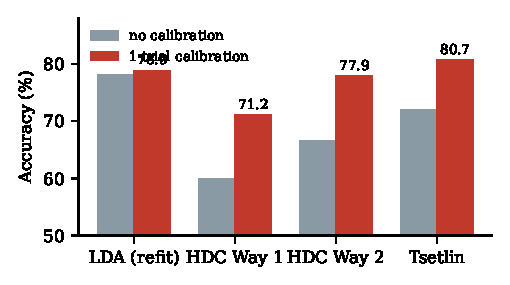
\includegraphics[width=\linewidth]{figures/calibration.pdf}
\caption{Accuracy before and after one-trial calibration (test: the user's other trials).}\label{fig:calib}
\end{figure}

\subsection{Calibration of the LDA itself}\label{sec:calib}
Simply refitting the LDA with one extra trial hardly moves it (+0.7\pp), because about 950 new
windows are added to some 50\,000. The team's adaptive LDA instead \emph{blends} the statistics:
\[
\mu_c\leftarrow(1-\lambda)\mu_c+\lambda\hat\mu_c^{\text{user}},\qquad
\Sigma\leftarrow(1-\lambda)\Sigma+\lambda\hat\Sigma^{\text{user}},
\]
then recomputes $W$ and $b$ in closed form. On the hardest subject (S15) this raised accuracy from
59.3\% to \textbf{89.5\%} with one trial, and to 89.9\% with two (INT8). This is the strongest
single argument for LDA on the chip: the calibration costs a few matrix operations on the host,
and the chip only reloads $W$ and $b$ through its configuration port. It has so far been measured
on one subject; extending it to all subjects is the first item of future work.

\subsection{Compute-in-memory}
A bit-serial digital CIM version of Stage 3 was analysed but not built. Each input is split into
bit-planes, $x=-2^7x_7+\sum_{b<7}2^bx_b$, so that
\[
\textstyle\sum_f W_fx_f=\sum_b c_b2^b\sum_f x_{f,b}W_f ,
\]
which needs only AND gates and an adder tree per class. That computes all six scores in 8 cycles
instead of $6(D+1)$. CIM saves energy when weight traffic dominates; here 720 weights are read
ten times a second, and the single MAC has spare time, so CIM would add area without benefit.

\subsection{Sequential decisions from correlated best-arm identification}\label{sec:ctbai}
A binary gesture decision can be posed as two-armed Gaussian best-arm identification. The arms are
the two class scores. Under the LDA model,
\[
\mathbb E[S_k\mid y]=-\tfrac12(\mu_k-\mu_y)^\top\Sigma^{-1}(\mu_k-\mu_y)+\text{const},
\]
so the arm with the highest mean is the true gesture. One window gives a \emph{joint pull}
$(S_1,S_2)$. The two scores are correlated, with
\[
\rho=\frac{w_1^\top\Sigma w_2}{\sqrt{w_1^\top\Sigma w_1\;w_2^\top\Sigma w_2}} ,
\]
which ranges from $-0.33$ to $+0.94$ across gesture pairs and varies widely between users, so it
must be treated as unknown. We applied the cost-weighted correlated stopping rules derived in the
team lead's bandit research:
\begin{itemize}
\item the GLR statistic with its non-asymptotic threshold;
\item the mixture-martingale statistic $W_t$ with threshold $\log(1/\delta)$.
\end{itemize}
Each rule was started after gesture onset and run on non-overlapping windows (Table~\ref{tab:ctbai}).

\begin{table}[t]\centering\small
\caption{Binary decisions, all 6 pairs pooled, $\delta=0.05$ (18 subjects). Undecided: no decision within about 6\,s of held gesture.}\label{tab:ctbai}
\resizebox{\linewidth}{!}{%
\begin{tabular}{lcccc}\toprule
Rule & Error & Undec. & Windows & Latency\\\midrule
1 window (today) & 6.60\% & 0\% & 1 & 0.20\,s\\
Vote of 5 & 5.86\% & 0\% & 5 & 1.00\,s\\
Mixture $W_t$ & 2.05\% & 12.5\% & 8.8 & 1.75\,s\\
GLR, $\rho$ unknown & 0.90\% & 34.7\% & 16.3 & 3.24\,s\\
GLR, $\rho=0$ & 0.28\% & 44.2\% & 10.6 & 2.10\,s\\
GLR, $\rho$ from training & 0.76\% & 30.6\% & 12.3 & 2.45\,s\\\bottomrule
\end{tabular}}
\end{table}

\begin{figure}[t]\centering
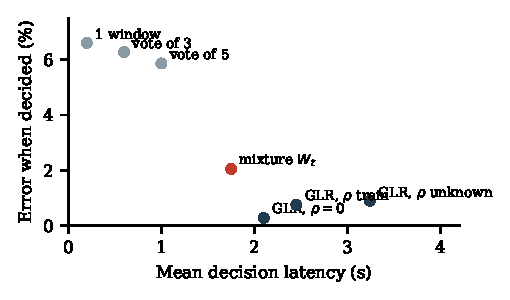
\includegraphics[width=\linewidth]{figures/stopping.pdf}
\caption{Error against latency for binary decisions ($\delta=0.05$; the GLR and mixture rules also leave some recordings undecided, Table~\ref{tab:ctbai}).}\label{fig:stop}
\end{figure}

\textbf{Observations.}
\begin{itemize}
\item On five of the six pairs, the mixture rule cuts the error to 0--1.1\% within under 2\,s.
\item Ignoring the correlation stalls the decision on strongly correlated pairs, as the theory
predicts: the $\rho=0$ rule decides 1\% of recordings on Hand Close vs Wrist Flexion, against 89\%
for the mixture rule.
\item The pair Hand Open vs Wrist Extension exceeds $\delta$ (12.6\%). The cause is classifier bias,
not the stopping rule: for some users the class means are in the wrong order, so the best arm is
the wrong gesture.
\end{itemize}

%=======================================================================
\section{Decisions and trade-offs}\label{sec:tradeoffs}
\begin{table*}[t]\centering\small
\caption{Every major decision, the alternatives considered, and the evidence.}\label{tab:decisions}
\begin{tabular}{p{2.3cm}p{2.8cm}p{3.7cm}p{7.0cm}}\toprule
Decision & Chosen & Alternatives & Reason / evidence\\\midrule
Evaluation & LOSO, trial-level validation, windows cut after the split & window-level split; per-subject training & only LOSO measures a new user; the window-level split leaked data (false 63\% ceiling)\\
Gesture set & HC, HO, WF, WE & Index/Index Little set; 6 or 12 gestures & +14.1\pp; finger gestures inseparable with 8 surface electrodes; 6 gestures 69.0\%\\
Classifier & INT8 LDA & MLP, LogReg, SVM, trees, CNN & all cheap linear models tied with the MLP; LDA has closed-form training and calibration and probabilistic scores; trees over budget or worse\\
Arithmetic & INT8 weights, INT32 accumulator, no requantisation & FP32; per-class scales & 0.18\pp\ mean loss; a shared scale keeps the argmax\\
Features & SABS, WL, ZC, SSC, Mitchell POW & float MAV/VAR/RMS, exact squares, log features & integer set matches the float reference; Mitchell square needs no multiplier\\
Normaliser & $(x-\mu)\gg k$, integer & z-score + float quantiser & no accuracy loss; only subtract, add and shift\\
Partition & 1 compute core + 1--3 ADC pods & multi-board partial sums; master/slave & one core handles up to 40 channels at 1\,MHz; distributing adds synchronisation for no gain\\
Stage 3 & 1 MAC, streaming argmax & parallel MACs; comparator tree; CIM & 850 of 1015 cycles at $C=24$; CIM saves nothing at 720 weights and 10\,Hz\\
Windows & 2 ping-pong banks of 98 & sliding sums; 2 write pointers & one write pointer; window = bank0 + bank1\\
Memories & writable RAM, 1-cycle read & ROM; flip-flops with combinational read & each channel count needs its own model; maps to SRAM or flip-flops\\
Clock crossing & toggle synchroniser for the event only & synchronise the data & data stable for about 1\,ms; one bit crosses\\
Verification & bit-exact golden model, unit and chip tests, injected bugs & accuracy-only checks & every intermediate value checked; injected bugs caught\\
New user & calibration (blended LDA statistics) & none; Tsetlin or HDC on chip & +30\pp\ on the worst subject with one trial; reuses the chip's config port\\\bottomrule
\end{tabular}
\end{table*}

Table~\ref{tab:decisions} lists every decision. Three trade-offs shaped the design most.
\begin{enumerate}
\item \textbf{Accuracy vs vocabulary.} Each added gesture costs accuracy. We favoured a reliable
4-gesture interface over a 12-gesture one at 49\%.
\item \textbf{Fixed function vs flexibility.} The on-chip LDA gives a self-contained, low-power
decision; the microcontroller variant trades that for classifier freedom.
\item \textbf{Latency vs reliability.} A decision every 100\,ms is fast but errs on about 6\% of
windows in a binary choice; a sequential rule errs about ten times less at about 1.8\,s.
\end{enumerate}

%=======================================================================
\section{Conclusion and future work}
Measured, subject-independent experiments justified each step. Gesture selection mattered most,
model capacity did not, integer arithmetic and INT8 cost almost nothing, and a one-multiplier core
at 1\,MHz is enough for 24 electrodes. The RTL is verified bit-exactly against a model whose
accuracy matches the software reference. Future work:
\begin{enumerate}
\item evaluate the blended-statistics LDA calibration on all subjects;
\item synthesise in a target process to report area and power;
\item run the sequential decision rule on the host or MCU, with a classifier calibrated per user
to remove the bias seen on Hand Open vs Wrist Extension;
\item extend the bandit theory to unknown, unequal variances, which this application needs.
\end{enumerate}

\appendix
\onecolumn
\section{Reproducing the results}
All commands run from the repository root; each script prints the tables quoted above.
\begin{center}\small
\resizebox{\linewidth}{!}{%
\begin{tabular}{lll}\toprule
Result & Script & Subjects\\\midrule
Gesture sets, classifiers, INT8 loss & \texttt{analysis/classifier\_classification.py}, \texttt{K\_4\_model\_MLP.py}, \texttt{K\_6\_model\_LR\_comparison.py} & 19\\
Integer features H1--H6 & \texttt{analysis/K\_4\_LDA\_HW\_Experiments.py} & 18\\
Feature-type selection & \texttt{analysis/fors\_emg\_feature\_selection\_lda.py} & 18\\
Chip model vs software LDA & \texttt{golden\_model/K\_4\_LDA\_Golden\_LOSO.py} & 18\\
LDA calibration & \texttt{analysis/K\_4\_LDA\_Calib.py} & 18 (target S15)\\
HDC, calibration & \texttt{explorations/K\_4\_HDC\_Way1\_vs\_Way2.py}, \texttt{K\_4\_HDC\_Calib.py} & 18\\
Tsetlin machine & \texttt{explorations/K\_4\_TM\_Calib.py} & 18\\
Stopping rules & \texttt{explorations/K\_2\_CTBAI\_Stopping.py} & 18\\
RTL & \texttt{RTL/tb/test\_emg\_top.py} (set \texttt{CHANNELS}) & synthetic\\\bottomrule
\end{tabular}}
\end{center}

\onecolumn
\section{Selected script outputs}
Verbatim excerpts of the script printouts (18 subjects; the repository copy of the dataset lacks
Subject~1). The full text is in \texttt{docs/report/outputs/script\_outputs.txt}.
{\scriptsize\verbatiminput{outputs/script_outputs.txt}}

\end{document}
